\documentclass[10pt,a4paper]{article}
\usepackage[margin=18mm,top=15mm,bottom=17mm]{geometry}
\usepackage{amsmath,amssymb}
\usepackage{graphicx}
\usepackage{booktabs}
\usepackage{tabularx}
\usepackage{array}
\usepackage{enumitem}
\usepackage{natbib}
\usepackage[hidelinks]{hyperref}
\usepackage{microtype}
\usepackage[T1]{fontenc}
\usepackage[utf8]{inputenc}
\usepackage{lmodern}
\usepackage{xcolor}
\usepackage{titlesec}
\usepackage{tcolorbox}
\usepackage{caption}
\usepackage{float}
\usepackage{fancyhdr}

\graphicspath{{figures/}{../../../../results/figures/mode1_gate6b/}}
\captionsetup{font=footnotesize,labelfont=bf,skip=3pt}
\setlength{\parindent}{0pt}
\setlength{\parskip}{0.30em}
\setlength{\emergencystretch}{2em}
\setlist[itemize]{leftmargin=5mm,itemsep=1.5pt,topsep=2pt}
\setlist[enumerate]{leftmargin=6mm,itemsep=1.5pt,topsep=2pt}

\titleformat{\section}[hang]{\normalfont\large\bfseries}{\thesection.\ }{0pt}{}
\titlespacing*{\section}{0pt}{7pt}{3pt}
\titleformat{\subsection}[hang]{\normalfont\normalsize\bfseries}{\thesubsection\ }{0pt}{}
\titlespacing*{\subsection}{0pt}{5pt}{2pt}

\newcolumntype{L}[1]{>{\raggedright\arraybackslash}p{#1}}
\newcolumntype{C}[1]{>{\centering\arraybackslash}p{#1}}
\newcolumntype{Y}{>{\raggedright\arraybackslash}X}

\definecolor{reportblue}{RGB}{0,74,135}
\definecolor{reportgreen}{RGB}{16,112,64}
\definecolor{reportamber}{RGB}{160,92,0}

\newcommand{\evidencebox}[2]{%
  \begin{tcolorbox}[colback=#1!5!white,colframe=#1!70!black,boxrule=0.45pt,
    arc=1pt,left=5pt,right=5pt,top=3pt,bottom=3pt,before skip=4pt,after skip=4pt]
    \small #2
  \end{tcolorbox}}

\newcommand{\figureconclusion}[1]{%
  \begin{tcolorbox}[colback=blue!2,colframe=reportblue,boxrule=0.35pt,
    arc=1pt,left=4pt,right=4pt,top=2pt,bottom=2pt,before skip=3pt,after skip=0pt]
    \footnotesize\textbf{Scientific conclusion.} #1
  \end{tcolorbox}}

\pagestyle{fancy}
\fancyhf{}
\fancyhead[L]{\footnotesize Mode-I adaptive remeshing -- supervisor report}
\fancyhead[R]{\footnotesize 08 October 2026}
\fancyfoot[C]{\thepage}
\renewcommand{\headrulewidth}{0.3pt}

\begin{document}

\begin{center}
  {\Large\textbf{Corrected Mode-I Adaptive Remeshing: Localization and Fracture-Response Verification}}\\[0.30em]
  {\large\textbf{Focused Supervisor Report -- 08 October 2026}}\\[0.25em]
  {\normalsize\textbf{Pruthviraja Reddy Vandavagali} (Matr. Nr. 68865)}\\[0.10em]
  {\footnotesize Master Thesis in Computational Materials Science -- Chair of Applied Mechanics (IMFD), TU Bergakademie Freiberg}
\end{center}
\vspace{-0.3em}
\hrule height 0.6pt

\section{Objective and decision context}

The purpose of this short report is to answer one focused question: \emph{did the corrected native Abaqus remeshing workflow localize refinement to the Mode-I crack-propagation corridor while preserving an acceptable fracture response?} The work therefore has three objectives:

\begin{enumerate}
  \item identify why the earlier adaptive mesh refined too much of the domain;
  \item demonstrate the corrected, crack-path-localized mesh; and
  \item verify the corrected mesh using reaction force, initial stiffness, spatial damage, and energy evidence.
\end{enumerate}

\evidencebox{reportgreen}{\textbf{Main outcome.} The earlier Step-1/pre-peak remeshing state produced broad refinement, whereas the later Step-2 stress-error field produced a narrow horizontal corridor through a posteriori localization-guided remeshing. The governed ET1 corrected mesh contains $14{,}483$ finite elements ($64.12\%$ in the corridor). It is only $+0.279\%$ away from the spatial-fine adaptive reference in $F_{\max}$ ($-1.856\%$ vs the paper-matched fixed benchmark) and preserves initial stiffness to $-0.0261\%$.}

\begin{table}[H]
\centering
\caption{Supervisor-facing status at the start of the 08 October meeting.}
\small
\begin{tabularx}{\textwidth}{L{2.6cm}L{3.1cm}Y}
\toprule
Topic & Status & Evidence-based interpretation \\
\midrule
Earlier adaptive mesh & Superseded for localization assessment & Native remeshing worked, but the selected Step-1 field drove broad refinement. \\
Corrected Step-2 mesh & Verified & Refinement follows the horizontal ligament and avoids refinement on the initial slit flanks. \\
Mechanical response & Verified over tested cases & $K_0$, $F_{\max}$, $u_{\mathrm{peak}}$, and crack symmetry remain stable: ET1 is within $+0.28\%$ of the spatial-fine adaptive reference and $-1.86\%$ of the fixed benchmark anchor. \\
Energetic interpretation & Qualified with limitation & Component histories are available; the exact global energy identity remains not yet closed. \\
Gate status & Ready for supervisor sign-off & Gate 6C, Mode-II, and Gate 7 remain on hold until a formal decision. \\
\bottomrule
\end{tabularx}
\end{table}

This report deliberately omits the detailed gate ledger, long derivations, intermediate failed packages, and full job history. Those remain in the governed project records.

\clearpage
\section{Problem with the earlier adaptive mesh}

The earlier native adaptive mesh was operational, but it was not an efficient representation of the intended fracture process zone. The $1\%$ target-error case contained $71{,}320$ finite elements and refined a large part of the specimen rather than concentrating resolution primarily along the future horizontal crack path. Figure~\ref{fig:legacy_mesh} retains only the requested full-domain and crack-tip views of that case.

\begin{figure}[H]
  \centering
  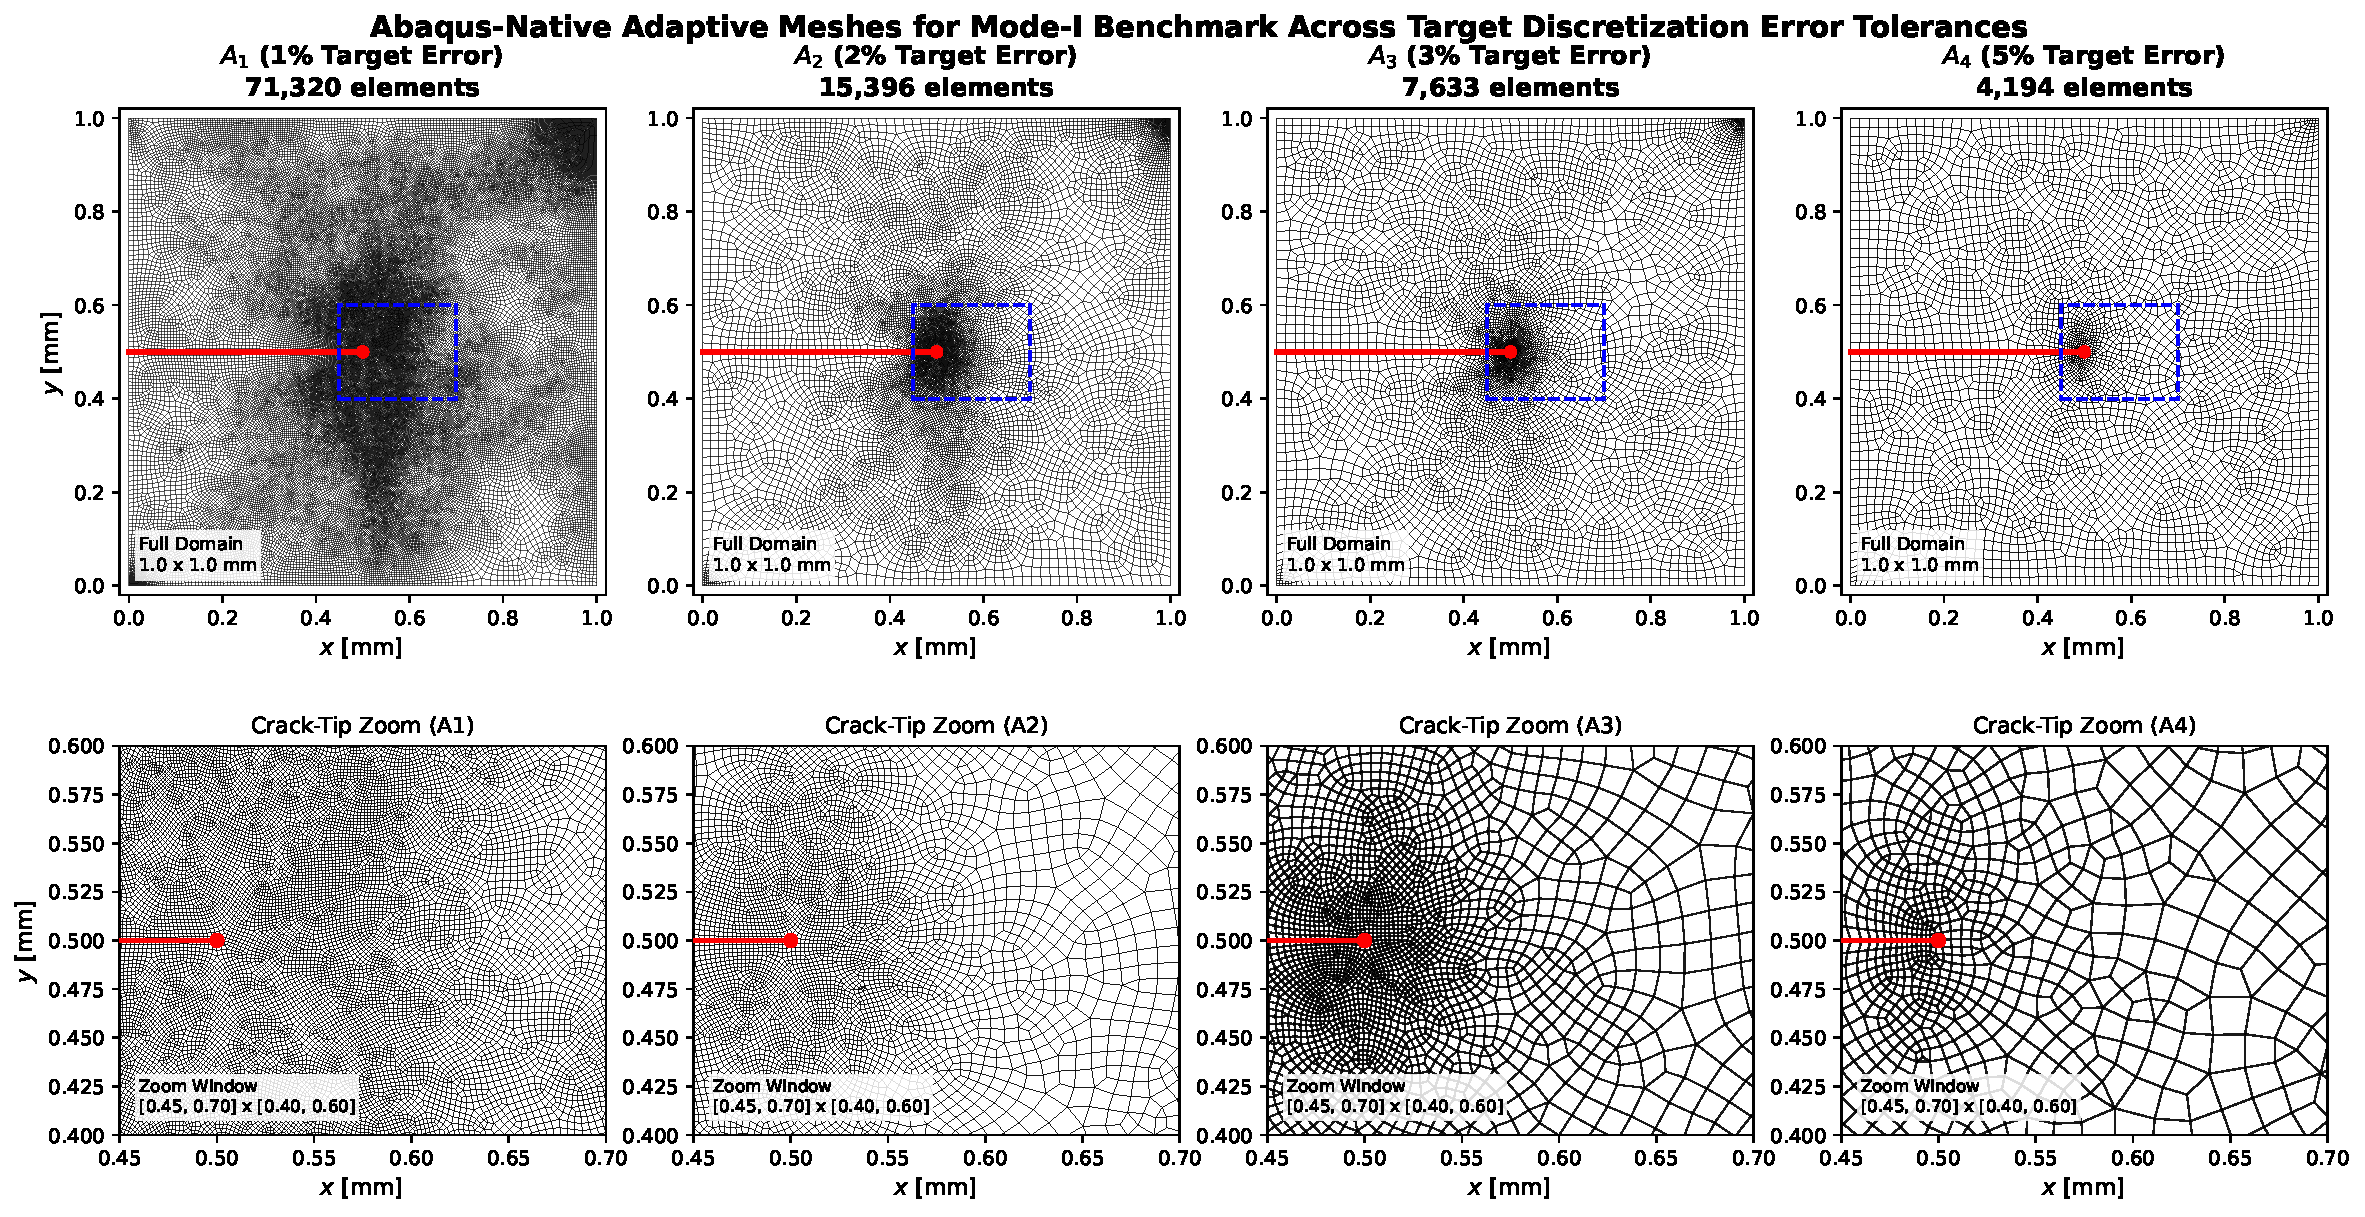
\includegraphics[width=0.48\textwidth,viewport=0 0 298 562,clip]{fig_adaptive_meshes_comparison.pdf}
  \caption{Earlier $71{,}320$-element Step-1/pre-peak adaptive mesh: full-domain view (top) and crack-tip zoom (bottom). Although the crack tip is refined, fine resolution is distributed broadly through the specimen.}
  \label{fig:legacy_mesh}
  \figureconclusion{Element count alone was not a sufficient quality measure. The central problem was spatial selectivity: too much resolution was placed away from the propagating ligament.}
\end{figure}

The broad pattern had two distinct issues that must not be conflated. First, an early boundary-set formatting defect omitted bottom-edge constraints and distorted stiffness; that defect was corrected and closed. Second, even with correct boundary conditions, the remeshing field had been evaluated at a Step-1/pre-peak state, before the fracture process had localized along the ligament. The second issue explains the inefficient mesh morphology addressed here.

\clearpage
\section{Corrections introduced}

The decisive change was to align the remeshing evaluation state with the physical feature that the mesh is intended to resolve. The native \texttt{RemeshingRule} now evaluates the localized Step-2 companion \texttt{MISESERI} field. This is a stress-error indicator, not the phase-field damage variable.

\begin{table}[H]
\centering
\caption{Difference table: earlier state, implemented correction, and observed effect.}
\footnotesize
\begin{tabularx}{\textwidth}{L{2.6cm}Y Y Y}
\toprule
Item & Earlier state / issue & Correction applied & Observed effect \\
\midrule
Remeshing evaluation state & Step-1/pre-peak field emphasized the initial crack-tip neighborhood and broad background error. & Use the \texttt{MISESERI} field evaluated during Step-2, after damage localization has developed, to generate a refined mesh along the Mode-I crack-propagation ligament. & Refinement extends along the horizontal ligament instead of filling most of the domain. \\
Quality criterion & Total element count received excessive emphasis. & Judge corridor share, band width, far-field fraction, crack symmetry, and response together. & Mesh efficiency is assessed by physical localization rather than count matching alone. \\
Tolerance study & A single tolerance could hide morphology sensitivity. & Evaluate \texttt{errorTarget} $\in\{1,2,3,5\}\%$ with identical bounds and region. & ET1 is target-like; ET2--ET5 progressively lose ligament resolution. \\
Post-processing & Results were dispersed across separate checks. & Use single-job provenance for RF--$u$, $K_0$, energy, phase field, and crack-path metrics. & Mechanical and spatial conclusions can be traced to exact jobs without cross-copying. \\
\bottomrule
\end{tabularx}
\end{table}

\evidencebox{reportamber}{\textbf{Scientific qualification.} The Step-1 field is evaluated at $u=0.005\,\mathrm{mm}$ and the Step-2 field at $u=0.010\,\mathrm{mm}$: both loading and localization states change, so the comparison does not isolate the step alone. The refined mesh is informed by an already developed crack pattern, and the fracture problem is solved again from its initial state. This is \emph{a posteriori localization-guided remeshing}. The $64.12\%$ corridor share demonstrates spatial refinement localization; it does not by itself establish prediction of an unknown crack path.}

\begin{figure}[H]
  \centering
  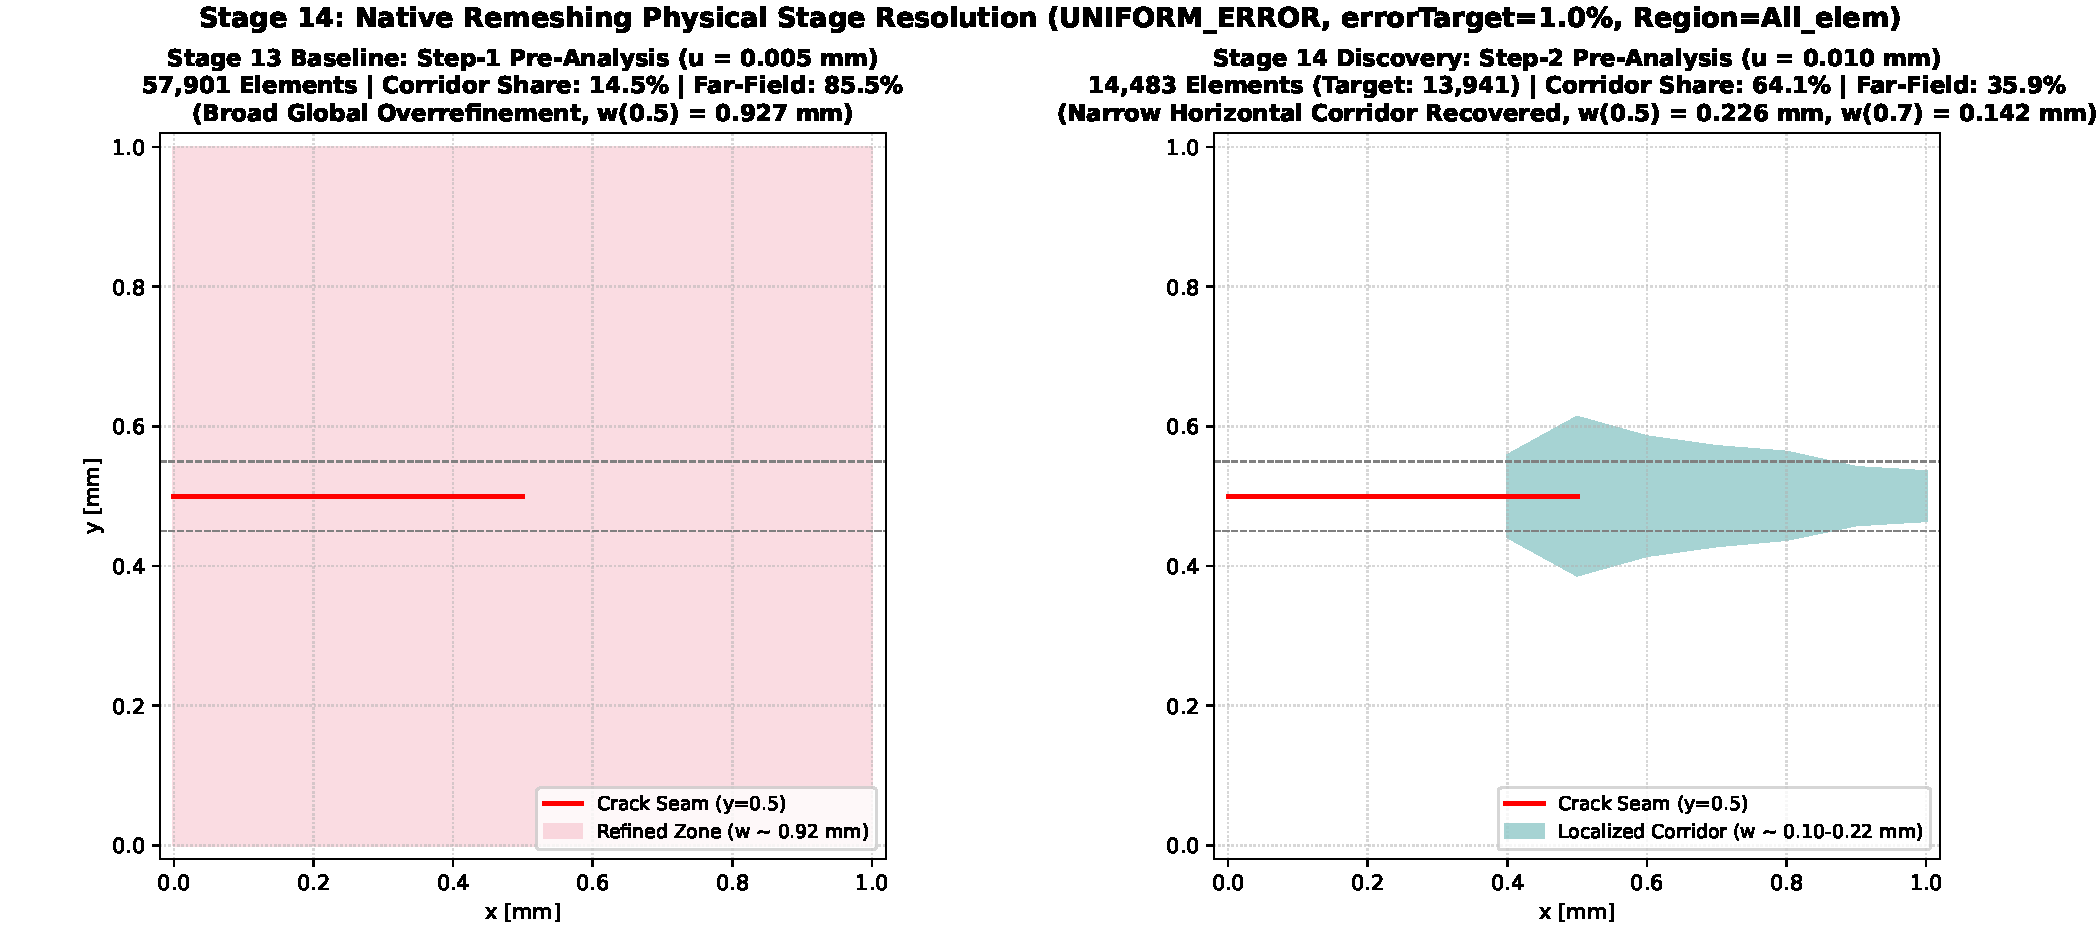
\includegraphics[width=0.98\textwidth]{fig_mode1_stage14_adapted_mesh_comparison.pdf}
  \caption{Comparison of loading and localization states at \texttt{errorTarget=1\%}. The historical Stage-13/Step-1 morphology (left) has exactly $57{,}901$ elements ($56{,}351$ CPE4 $+1{,}550$ CPE3; deck SHA-256 \texttt{872B54A6\ldots}) and produces broad global refinement. It is distinct from the later $57{,}929$-element spatial-fine fracture candidate. The corrected Step-2 ET1 mesh (right) has $14{,}483$ elements, $64.1\%$ corridor share, and $35.9\%$ far-field share.}
  \label{fig:stage_selection}
  \figureconclusion{The later Step-2 stress-error field produces a narrower refinement corridor. Loading state and damage localization both change; this comparison does not isolate the effect of step selection.}
\end{figure}

\clearpage
\section{Corrected adaptive mesh}

Figure~\ref{fig:corrected_mesh} shows the governed corrected ET1 mesh at both specimen and ligament scales. It contains $14{,}483$ finite elements ($14{,}082$ quadrilaterals and $401$ triangles) and $14{,}456$ finite-element nodes. The minimum and median area-equivalent element sizes are $0.760\,\mu\mathrm{m}$ and $2.597\,\mu\mathrm{m}$, respectively.

\begin{figure}[H]
  \centering
  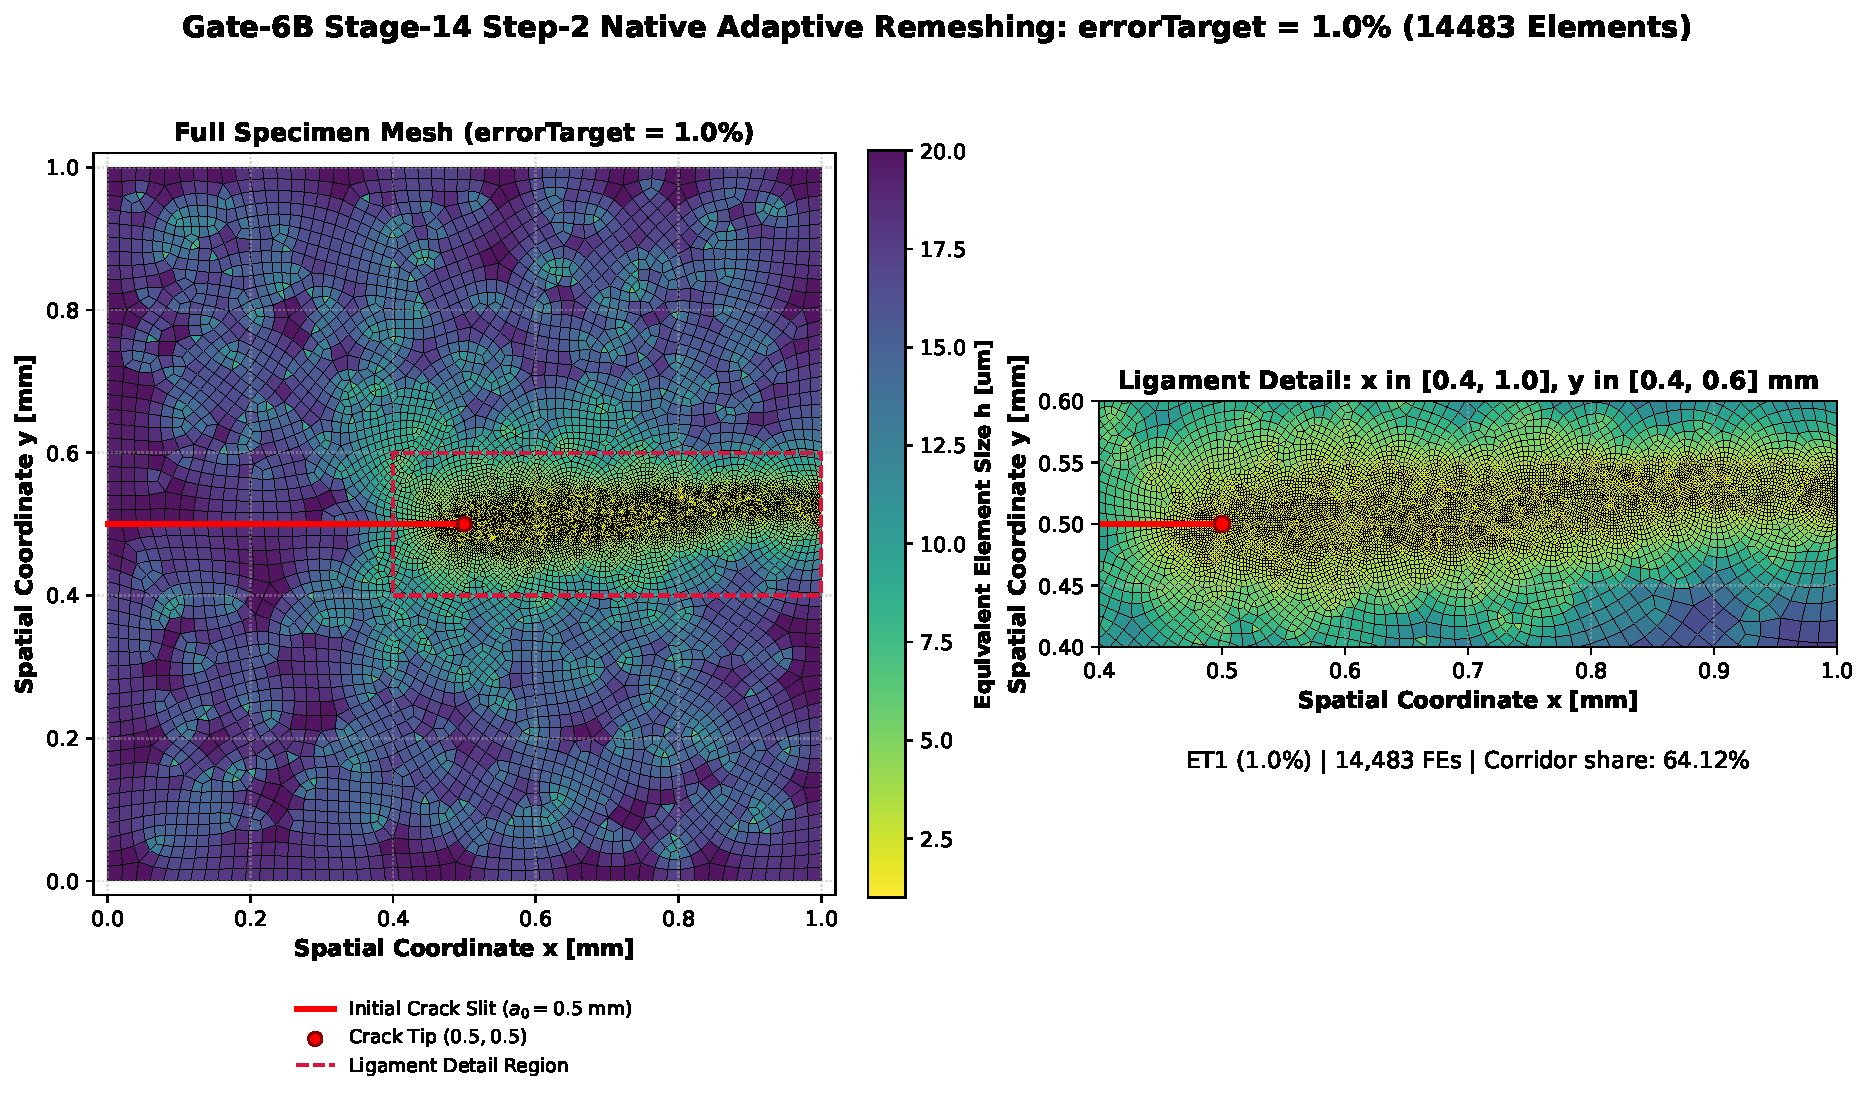
\includegraphics[width=0.99\textwidth]{Mode1_STAGE14_STEP2_ET1_14483.pdf}
  \caption{Corrected Step-2 ET1 adaptive mesh: full-domain view (left) and ligament zoom (right). The refined corridor begins at the initial crack tip and follows the expected horizontal propagation line. The mesh contains $14{,}483$ finite elements, with $64.12\%$ in the defined horizontal refinement corridor; $h_{\min}=0.760\,\mu\mathrm{m}$ and $h_{\mathrm{median}}=2.597\,\mu\mathrm{m}$. The initial slit flanks at $x\le0.3\,\mathrm{mm}$ show zero artificial refinement in the governed width metric.}
  \label{fig:corrected_mesh}
  \figureconclusion{The corrected mesh concentrates its finest resolution in the physically relevant crack-propagation region while retaining a comparatively coarse far field.}
\end{figure}

The morphology is qualitatively consistent with the localized adaptive pattern reported by \citet{pandey2025}. This statement concerns the character of the refinement corridor, not an exact reproduction of their reported $13{,}941$ elements. The publication does not expose enough implementation detail to establish exact count identity.

\clearpage
\section{Mesh roles and tolerance sensitivity}

The Step-2 error-target sweep separates localization quality from simple element reduction. All four tolerance cases use the same evaluation state, region, minimum/maximum size bounds, and coarsening policy; only the target tolerance changes.

\evidencebox{reportamber}{\textbf{Clarification of reference roles and benchmark semantics.} The $15{,}192$-element fixed case is the \textbf{paper-matched fixed benchmark anchor}: it reproduces the Pandey--Kumar published peak ($0.7578\,\mathrm{kN}$). Its role here is benchmark agreement, not a claim of an independently converged solution. The $57{,}929$-element case is the \textbf{internal adaptive convergence reference} (finest in the adaptive family). Corrected ET1 ($14{,}483$ FEs) is the preferred practical mesh. Historical Stage-13 ($57{,}901$ FEs) is only a legacy demo of broad unlocalized refinement.}

\begin{table}[H]
\centering
\caption{Comparison of corrected Step-2 tolerance cases against the paper-matched fixed benchmark anchor and the spatial-fine adaptive reference.}
\small
\setlength{\tabcolsep}{2pt}
\renewcommand{\arraystretch}{1.2}
\begin{tabularx}{\textwidth}{L{1.8cm}C{1.1cm}C{1.2cm}C{1.6cm}C{1.5cm}C{1.5cm}C{1.5cm}C{1.6cm}Y}
\toprule
Case & Base FE & Corridor share & $K_0$ \newline [kN/mm] & $F_{\max}$ \newline [kN] & $\Delta$ vs benchmark & $\Delta$ vs fine adaptive & $u_{\mathrm{peak}}$ \newline [mm] & Role / Purpose \\
\midrule
Fixed benchmark & $15{,}192$ & --- & $137.9455$ & $0.757778$ & $0.000\%$ & $+2.177\%$ & $0.005857$ & Benchmark anchor \\
ET1 ($1\%$) & $14{,}483$ & $64.12\%$ & $137.9096$ & $0.743701$ & $-1.856\%$ & $\mathbf{+0.279\%}$ & $0.005733$ & Preferred ET1 \\
ET2 ($2\%$) & $6{,}112$ & $41.07\%$ & $137.9761$ & $0.756367$ & $-0.186\%$ & $+1.987\%$ & $0.005841$ & Tolerance study \\
ET3 ($3\%$) & $5{,}189$ & $34.59\%$ & $137.9775$ & $0.759407$ & $+0.215\%$ & $+2.397\%$ & $0.005876$ & Tolerance study \\
ET5 ($5\%$) & $4{,}692$ & $27.51\%$ & $138.0091$ & $0.765400$ & $+1.006\%$ & $+3.205\%$ & $0.005926$ & Tolerance study \\
\textbf{Spatial-fine} & $\mathbf{57{,}929}$ & --- & $\mathbf{137.8410}$ & $\mathbf{0.741633}$ & $\mathbf{-2.131\%}$ & $\mathbf{0.000\%}$ & $\mathbf{0.005717}$ & \textbf{Convergence ref.} \\
\bottomrule
\end{tabularx}
\end{table}

Two distinct comparisons are provided in Table~3. The benchmark reference assesses agreement with the paper-matched fixed-mesh solution, while the spatial-fine adaptive reference assesses convergence within the adaptive discretization family.

ET1 differs from the spatial-fine adaptive reference by only $+0.279\%$ in $F_{\max}$ while using approximately $75\%$ fewer elements. The $-2.131\%$ peak difference between the spatial-fine reference and the fixed benchmark remains an unresolved benchmark offset.

\clearpage
\section{Mechanical verification: reaction force and energy}

Figure~\ref{fig:global_synthesis} compares three distinct scientific roles: the paper-matched fixed benchmark anchor ($15{,}192$ FE), the corrected ET1 adaptive mesh ($14{,}483$ FE), and the spatial-fine adaptive convergence reference ($57{,}929$ FE, Job \texttt{1410504.mmaster02}). The fine candidate was completed over the full $u=0.010\,\mathrm{mm}$ horizon using qualified 8-thread shared-memory execution.

\begin{figure}[H]
  \centering
  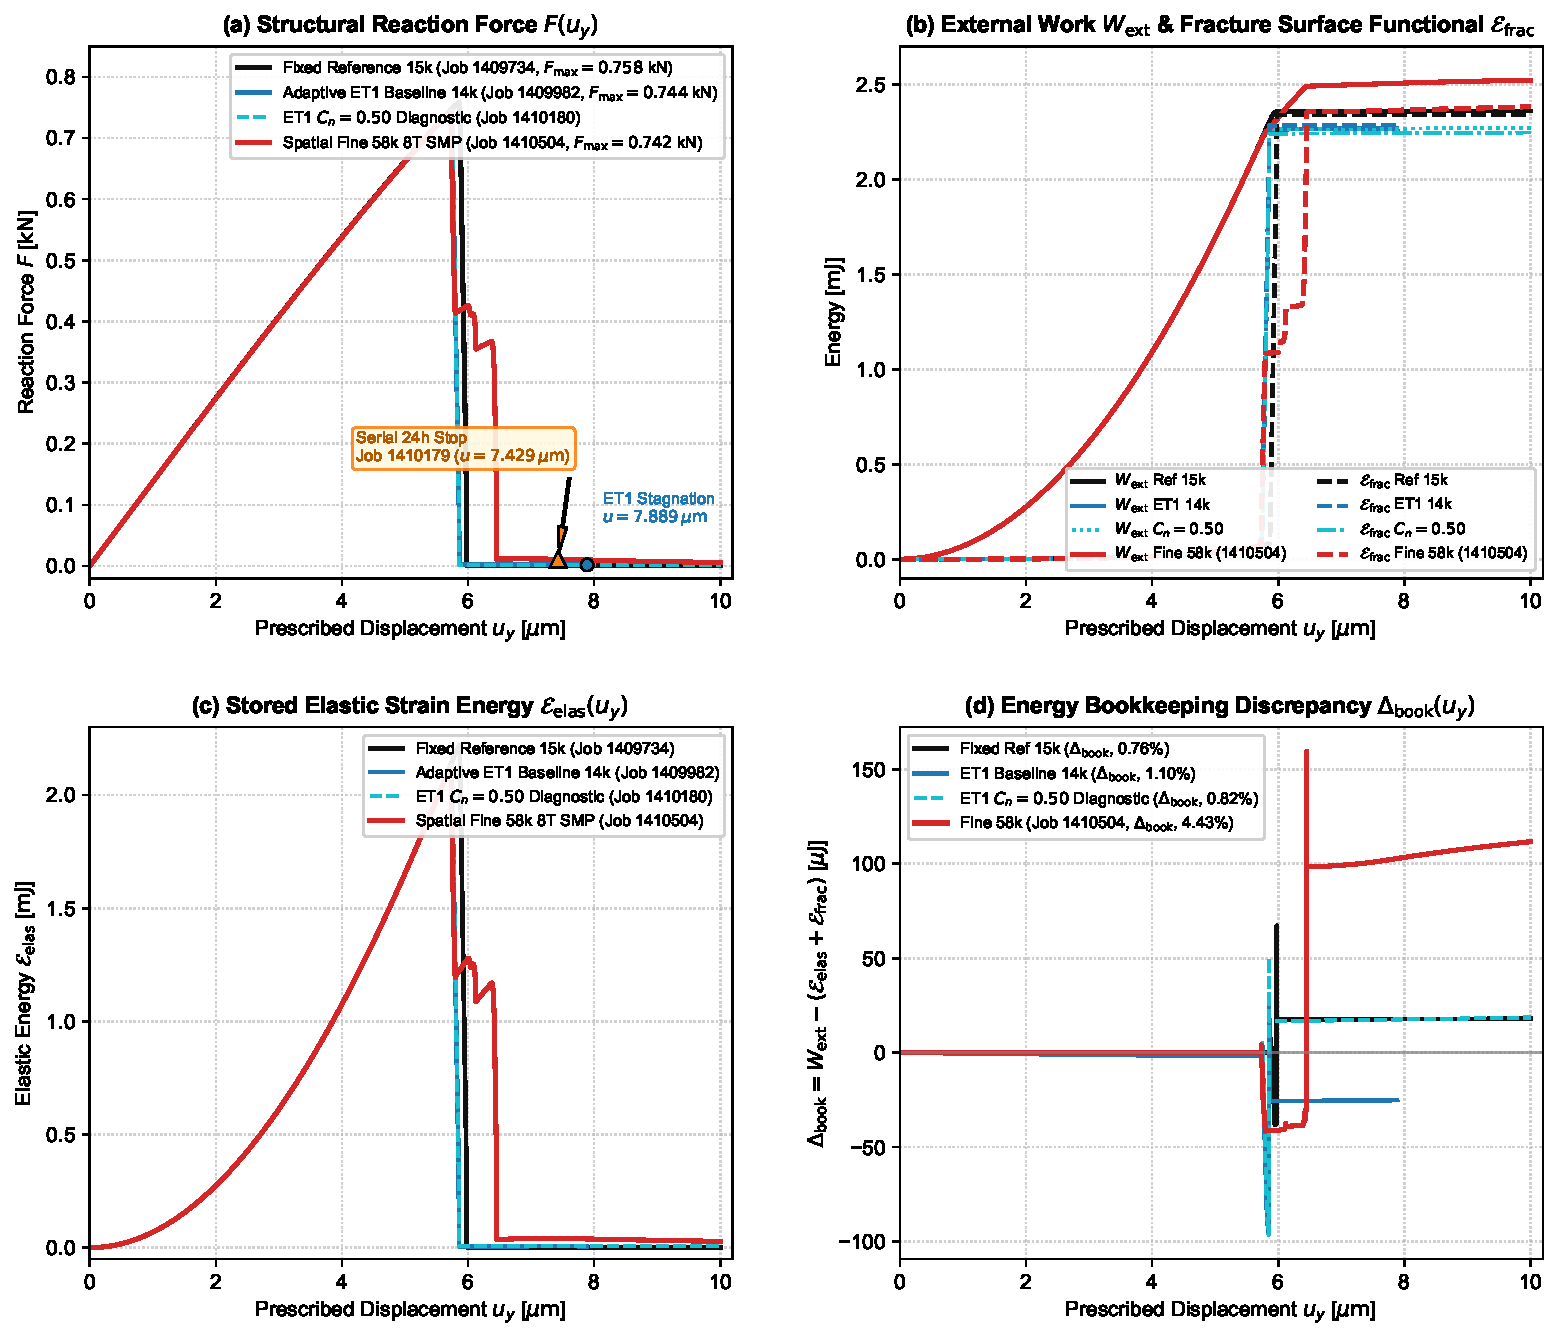
\includegraphics[width=0.88\textwidth]{fig_mode1_gate6b_spatial_convergence_synthesis.pdf}
  \caption{Three-case Gate-6B global synthesis: (a) reaction force; (b) external work and phase-field fracture-energy functional; (c) stored elastic energy; and (d) energy-bookkeeping difference. ET1 is censored at $u=0.007889\,\mathrm{mm}$ after a $98.5\%$ load drop; no values are forward-filled.}
  \label{fig:global_synthesis}
  \figureconclusion{The corrected adaptive meshes reproduce the elastic branch and peak response. The change from ET1 to the spatial-fine reference is only $+0.279\%$ in $F_{\max}$, confirming internal adaptive spatial convergence. The $-2.131\%$ peak difference relative to the fixed benchmark anchor represents an unresolved discretization-family offset, not an adaptive defect.}
\end{figure}

\begin{table}[H]
\centering
\caption{Compact result summary. Energies are compared only over each job's valid reached domain.}
\scriptsize
\begin{tabularx}{\textwidth}{L{3.0cm}rrrrrY}
\toprule
Case & Base FE & $K_0$ & $F_{\max}$ & $E_{\mathrm{frac}}$ & Energy residual $\varepsilon_{\mathrm{book}}$ & Valid domain / interpretation \\
 & & [kN/mm] & [kN] & [mJ] & [\%] & \\
\midrule
Fixed benchmark anchor & $15{,}192$ & $137.9455$ & $0.757778$ & $2.340220$ & $0.7607$ & Full horizon, $u=0.0100\,\mathrm{mm}$ \\
Corrected ET1 & $14{,}483$ & $137.9096$ & $0.743701$ & $2.285469$ & $1.1048$ & Reached $u=0.007889\,\mathrm{mm}$; $98.5\%$ load drop \\
Spatial-fine reference & $57{,}929$ & $137.8410$ & $0.741633$ & $2.381941$ & $4.4263$ & Full horizon, $u=0.0100\,\mathrm{mm}$ \\
\bottomrule
\end{tabularx}
\end{table}

Here $\varepsilon_{\mathrm{book}}=\left|W_{\mathrm{ext}}-(E_{\mathrm{elas}}+E_{\mathrm{frac}})\right|/|W_{\mathrm{ext}}|\times100\%$. Thus $4.4263\%$ is an endpoint energy-bookkeeping residual, not a fracture-energy error. The curves are physically bounded and the fine run closes the full displacement horizon, but this two-term residual is not proof of an exact joint potential for the staggered history-field algorithm. The global energy identity therefore remains formally not yet closed.

\clearpage
\section{Initial stiffness verification (\texorpdfstring{$K_0$}{K0})}

The initial elastic branch is the cleanest test of geometry, support conditions, material constants, and reference-point coupling. The canonical ordinary-least-squares fit uses the first $400$ increments up to $u\le0.0010\,\mathrm{mm}$.

\begin{figure}[H]
  \centering
  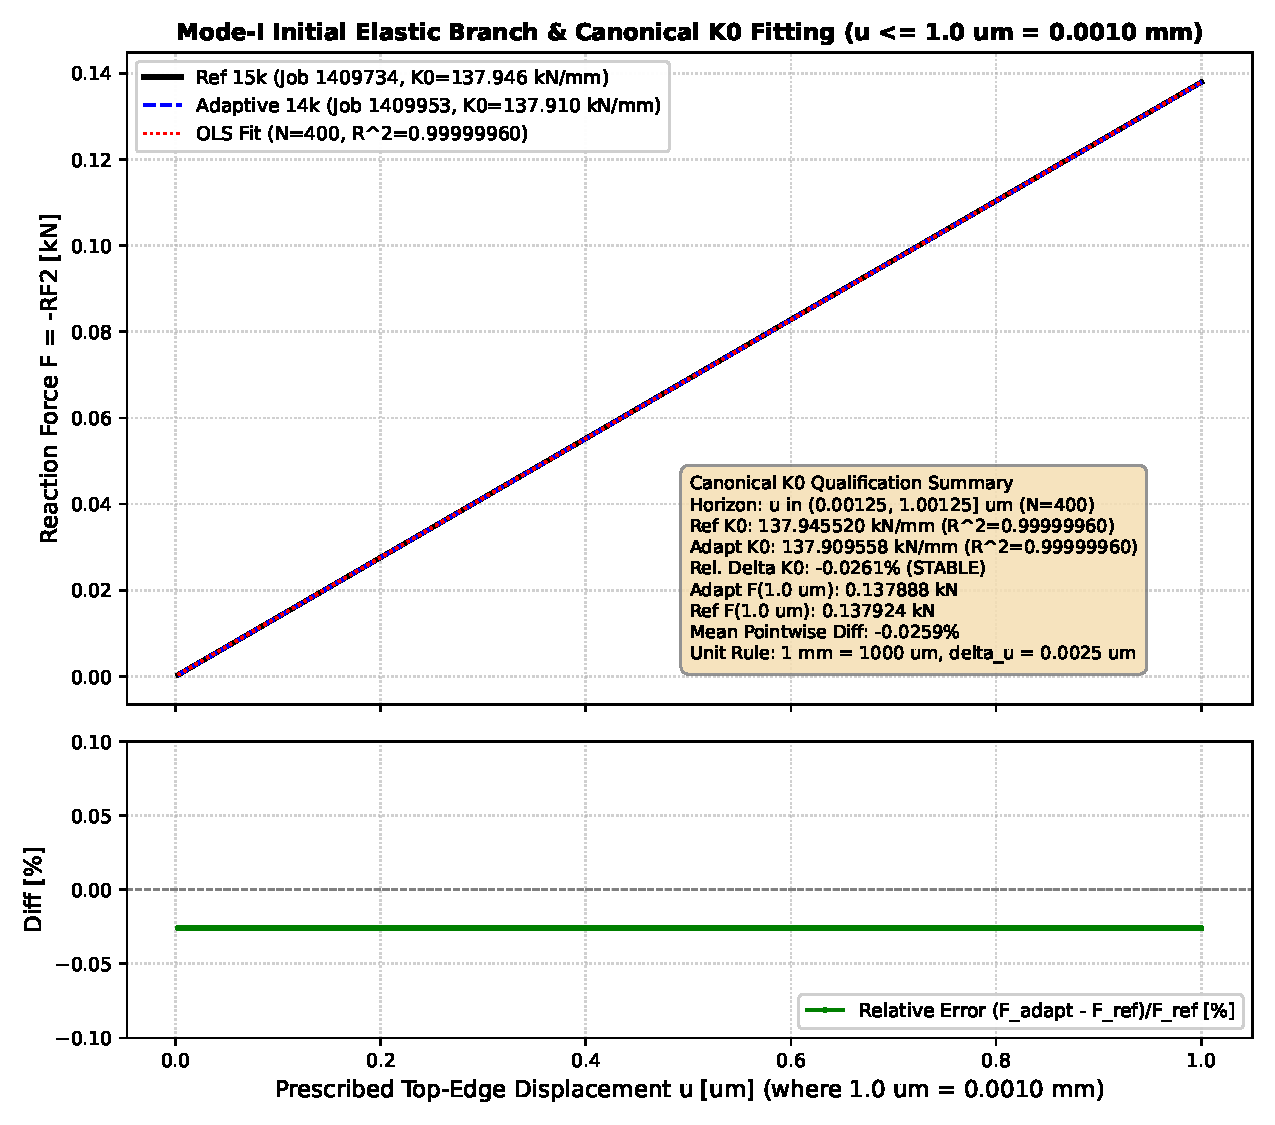
\includegraphics[width=0.84\textwidth,clip]{fig_mode1_stage14n_canonical_k0_fitting.pdf}
  \caption{Canonical $K_0$ comparison for the fixed benchmark anchor, corrected ET1, and spatial-fine adaptive reference. The fitted stiffnesses are $137.945520$, $137.909558$, and $137.840989\,\mathrm{kN/mm}$, respectively; both adaptive results remain within $0.08\%$ of the benchmark.}
  \label{fig:k0_fit}
  \figureconclusion{The corrected adaptive mesh preserves the initial structural response. The earlier boundary-condition defect is closed and initial stiffness is identical within $0.08\%$ across both discretization families.}
\end{figure}

The spatial-fine $57{,}929$-element candidate gives $K_0=137.840989\,\mathrm{kN/mm}$ ($-0.0758\%$ relative to the fixed benchmark anchor and $-0.0497\%$ relative to ET1), confirming stiffness stability across a fourfold change in adaptive element count.

\clearpage
\section{Spatial damage and crack-path verification}

Global RF--$u$ agreement is not sufficient by itself. The phase-field distribution must also remain centered on the Mode-I symmetry plane and progress along the intended ligament.

\begin{figure}[H]
  \centering
  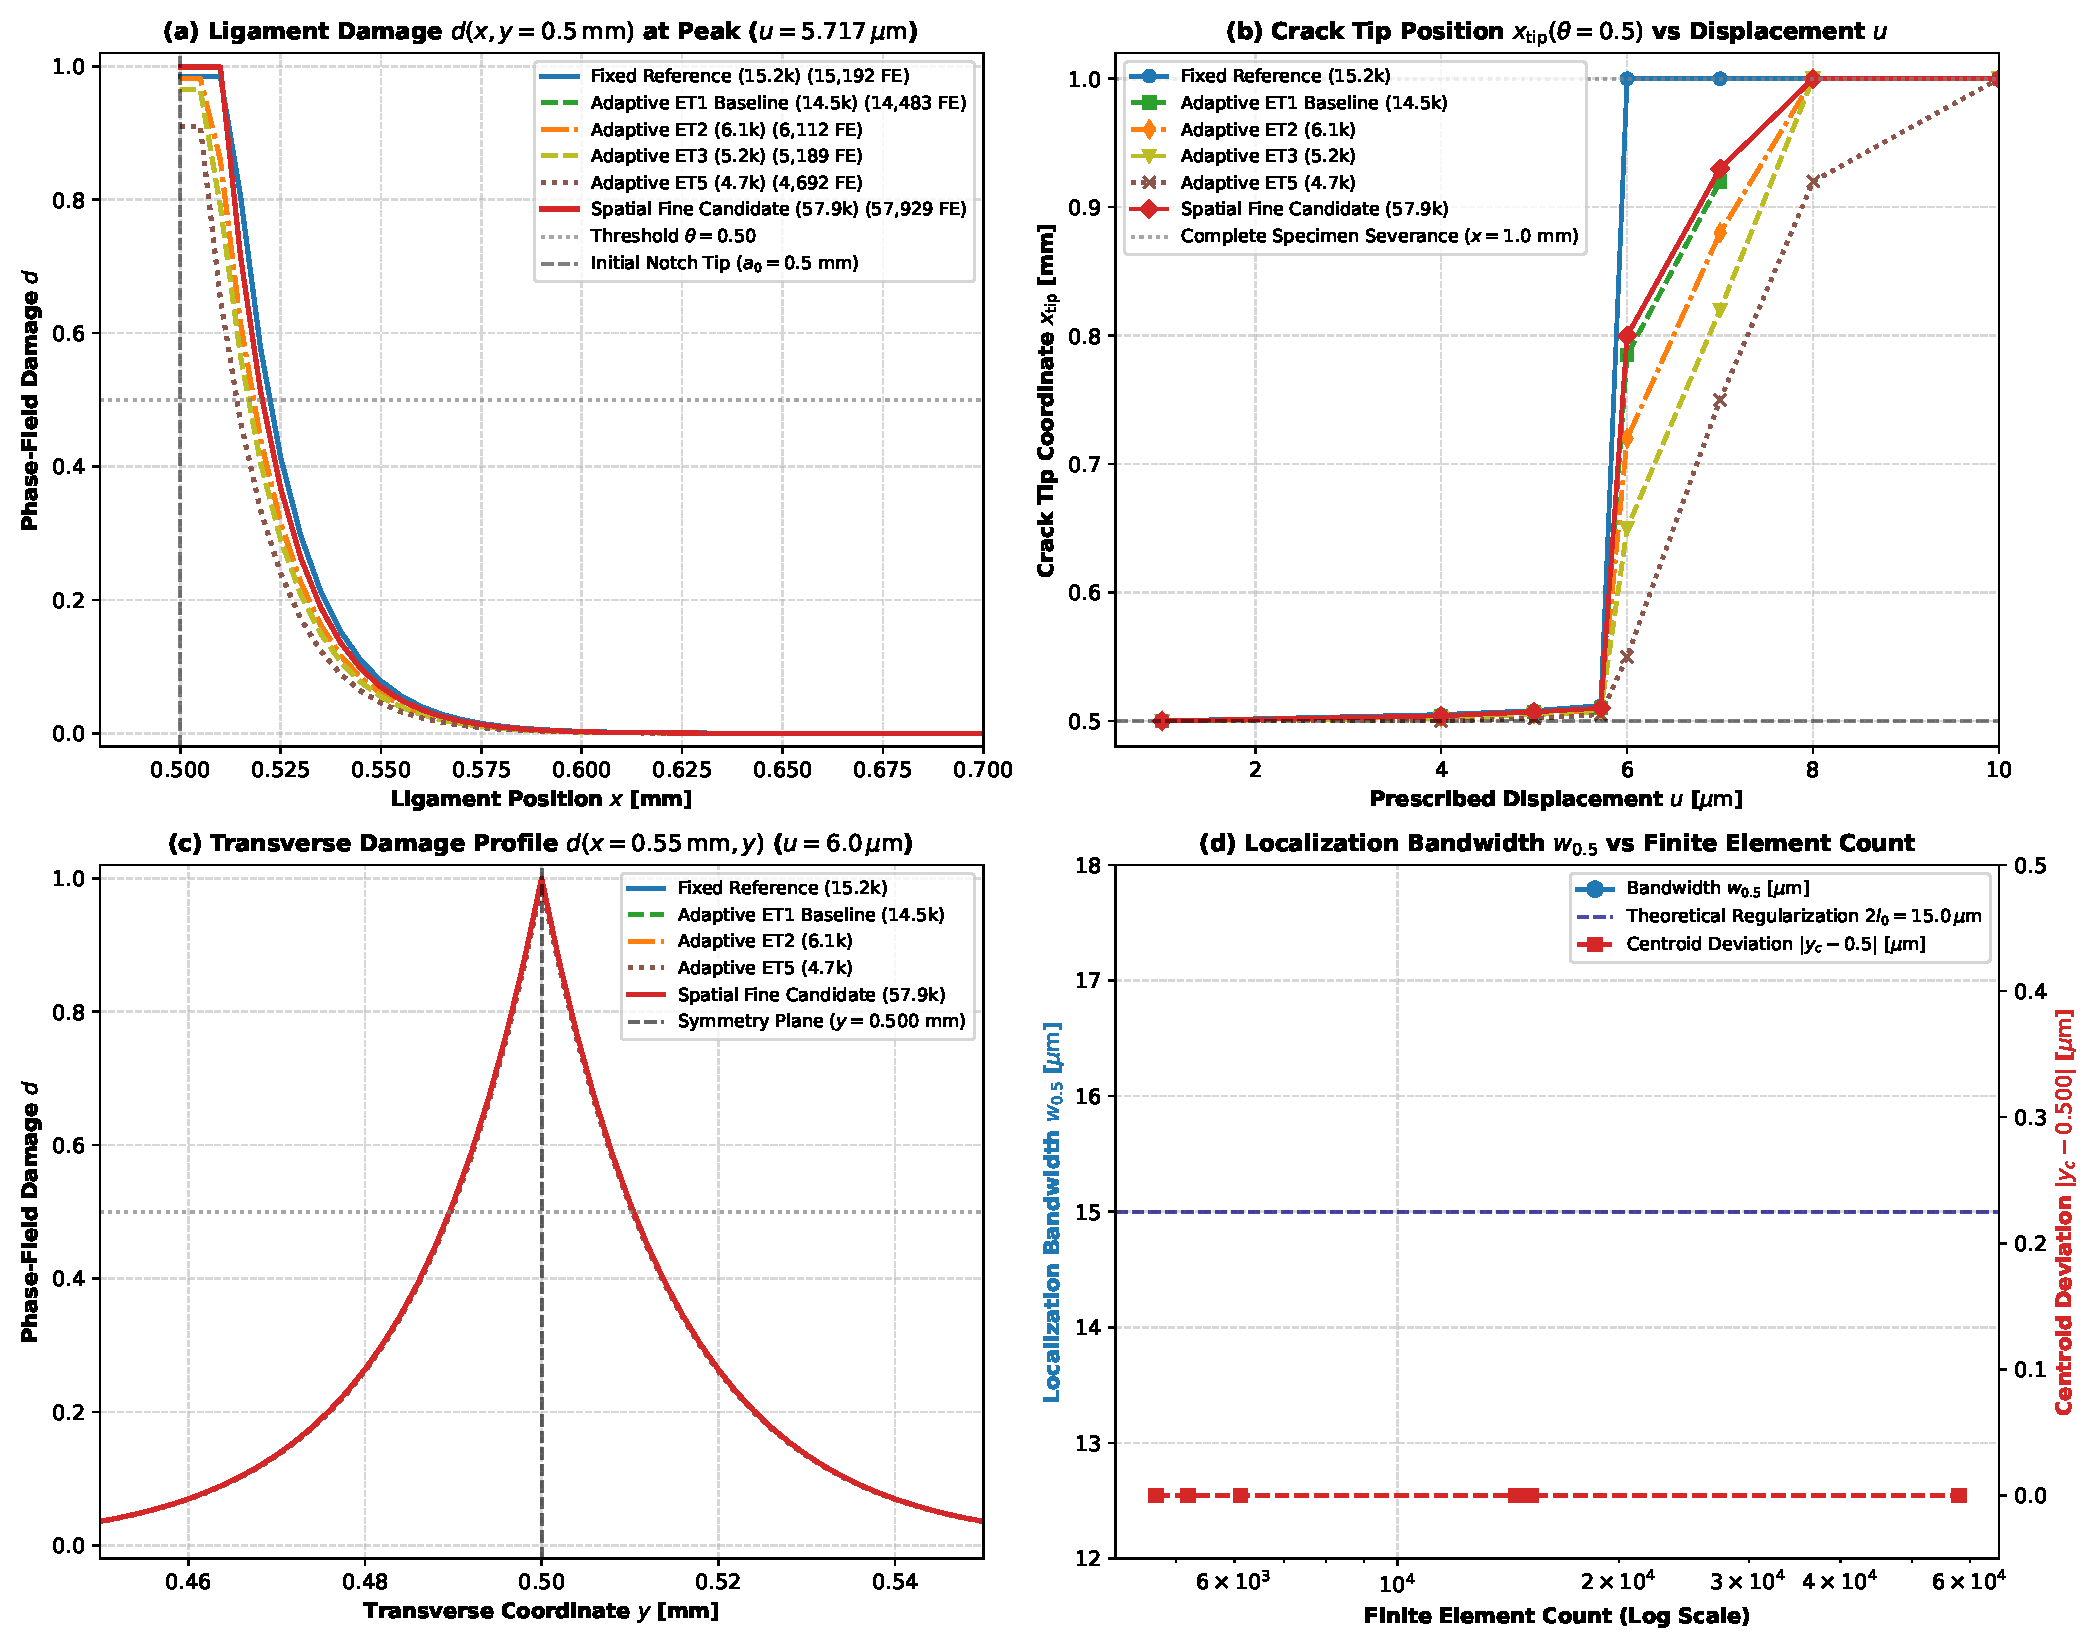
\includegraphics[width=0.87\textwidth]{fig_mode1_gate6b_spatial_localization_and_crack_path.pdf}
  \caption{Three-case spatial verification for the fixed benchmark anchor, corrected ET1, and spatial-fine adaptive reference: peak ligament profiles, crack-tip motion, transverse damage profiles, localization bandwidth, and centroid deviation.}
  \label{fig:spatial_localization}
  \figureconclusion{The corrected meshes preserve a horizontal Mode-I crack path. Pre-peak ET1 and spatial-fine ligament profiles differ by at most $0.32\%$ in the governed $L_2$ measure, and the transverse damage centroid remains at $y=0.500\,\mathrm{mm}$ within the evaluated precision.}
\end{figure}

The observed transverse localization bandwidth is approximately $w_{0.5}\approx15\,\mu\mathrm{m}$, close to the reference width $2l_0=15\,\mu\mathrm{m}$ for $l_0=7.5\,\mu\mathrm{m}$. This comparison is descriptive rather than an asserted analytical identity for the exact AT2 half-maximum profile. The mesh corridor remains wider than the observed damage band, so the regularized profile is resolved without forcing the crack path through a single row of elements.

\clearpage
\section{Matched phase-field contours}

Figure~\ref{fig:matched_contours} provides the requested spatial-field check at three matched displacements. It compares the fixed $15{,}192$-element benchmark anchor and corrected $14{,}483$-element ET1 adaptive mesh without using unmatched time frames.

\begin{figure}[H]
  \centering
  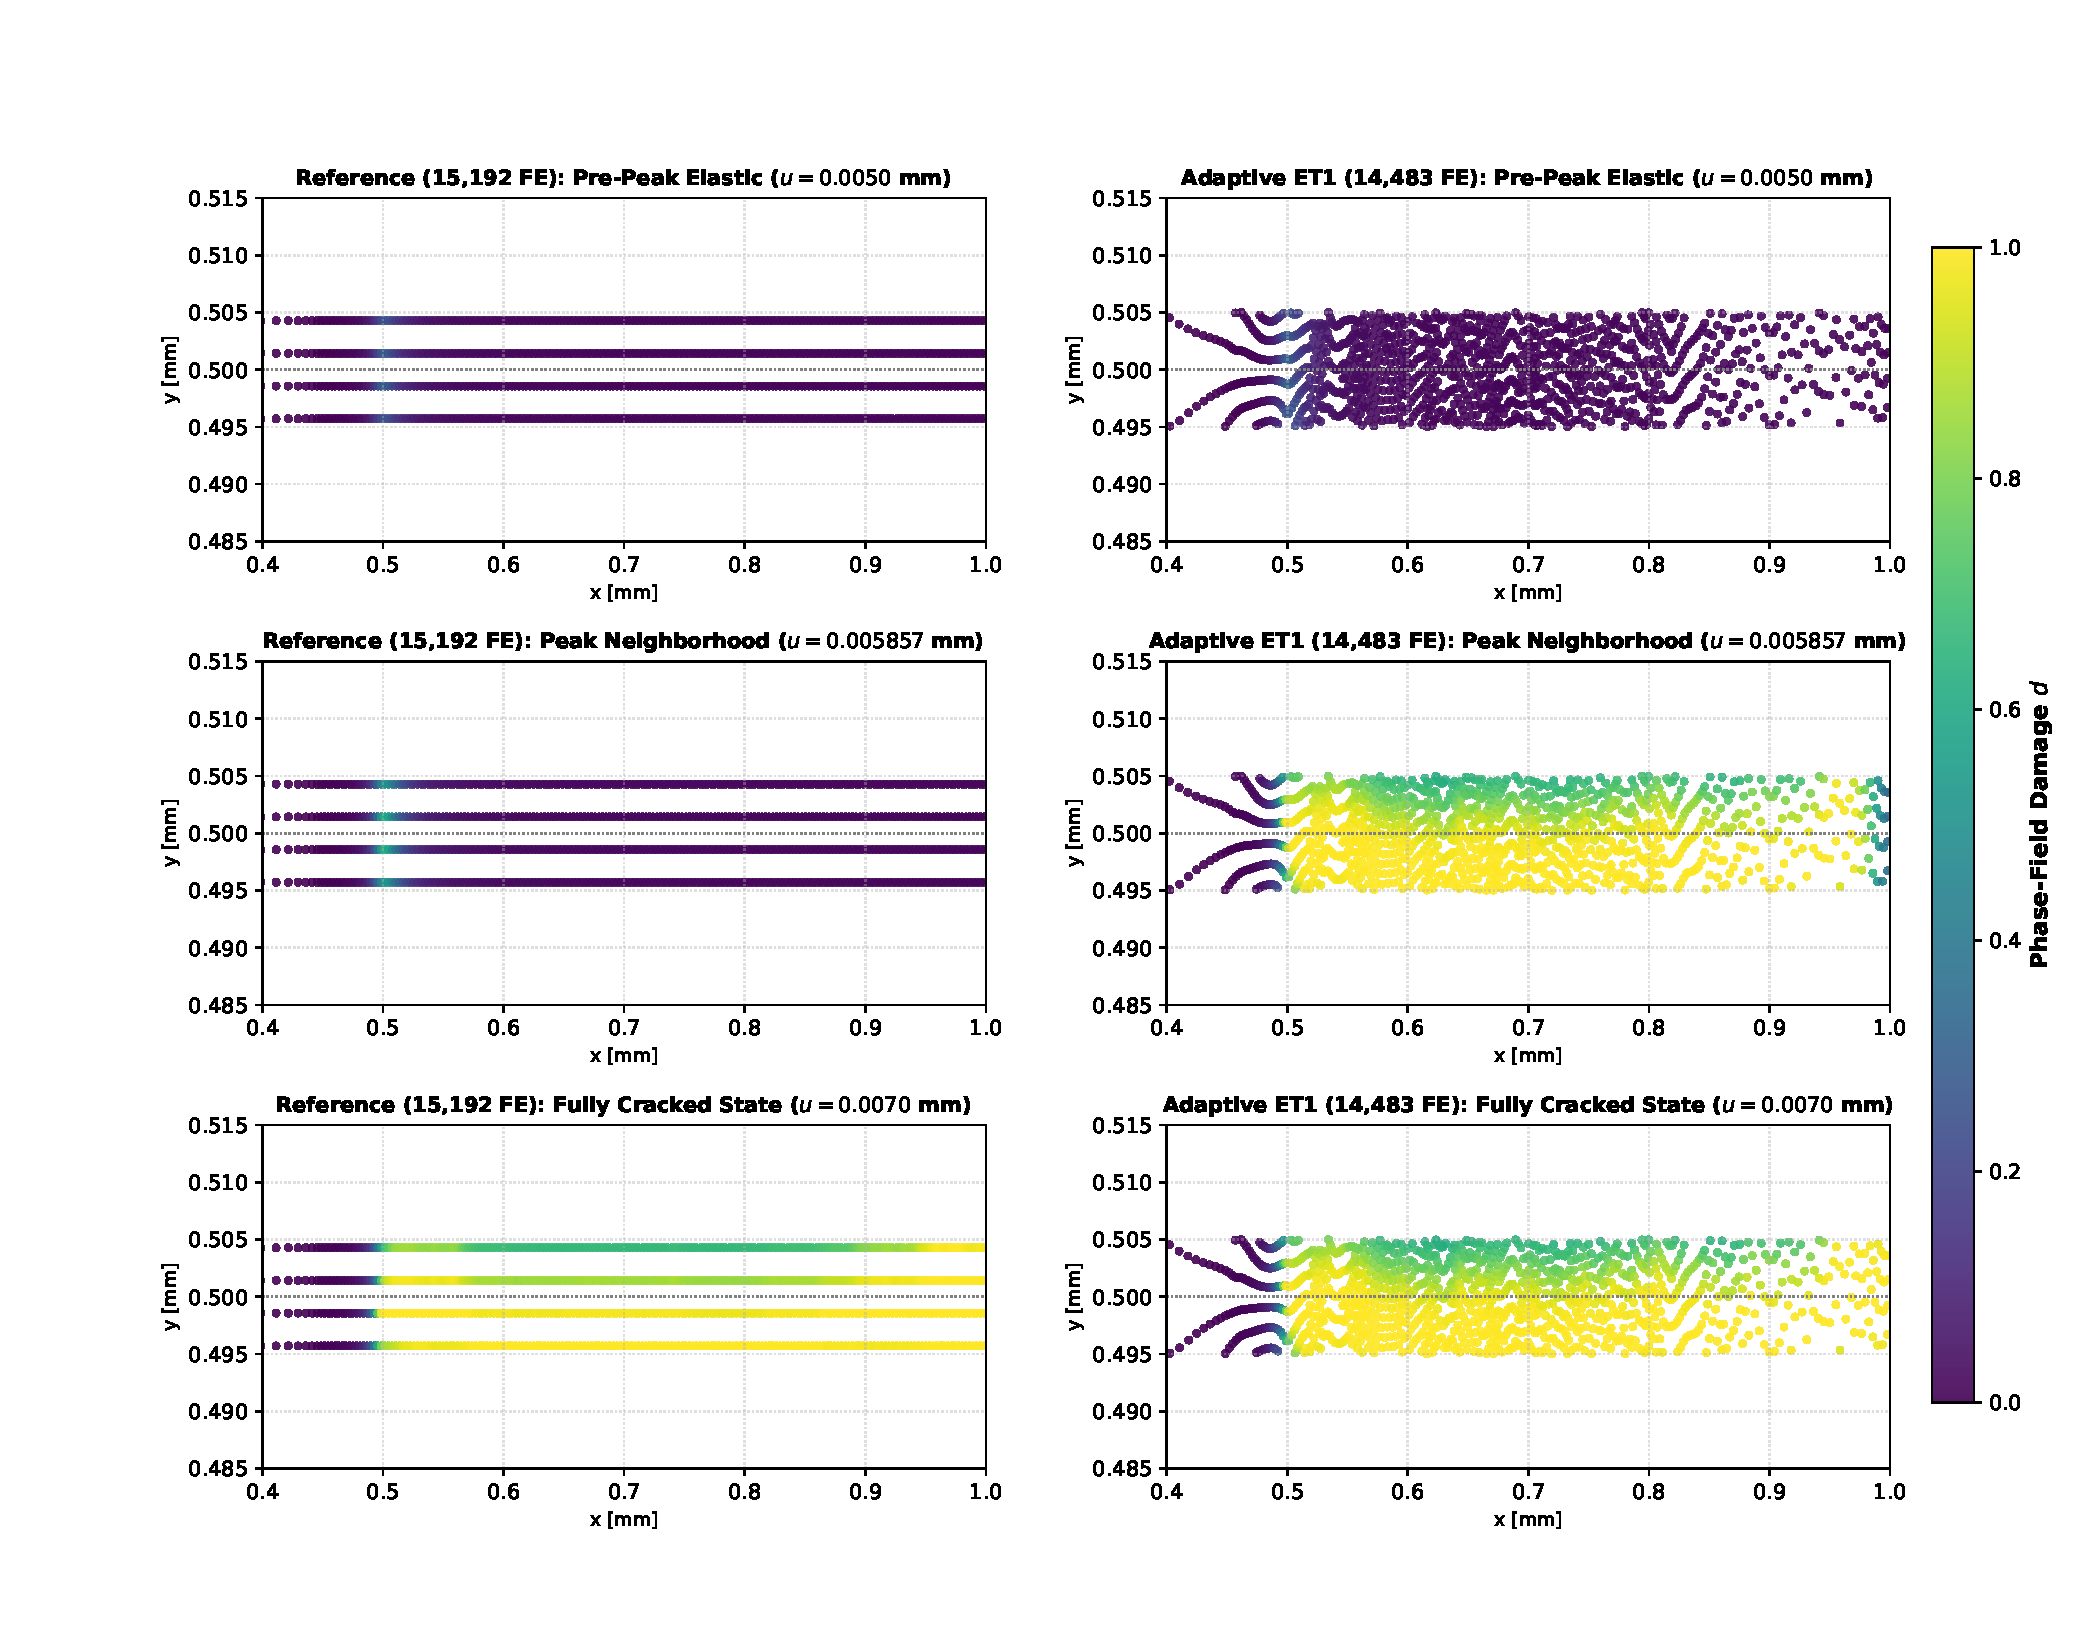
\includegraphics[width=0.87\textwidth]{fig_mode1_spatial_phase_field_contours_matched.pdf}
  \caption{Matched phase-field damage contours for the fixed benchmark anchor (left column) and corrected ET1 adaptive mesh (right column) at $u=0.0050\,\mathrm{mm}$, the reference peak neighborhood $u=0.005857\,\mathrm{mm}$, and the fully cracked state $u=0.0070\,\mathrm{mm}$.}
  \label{fig:matched_contours}
  \figureconclusion{The corrected adaptive solution localizes on the same horizontal ligament as the fixed benchmark anchor and reaches complete specimen separation without off-axis crack growth.}
\end{figure}

The point patterns differ because the benchmark uses a structured corridor while the adaptive mesh is unstructured. The scientifically relevant comparison is therefore the field distribution and crack trajectory, not node-by-node visual identity.

\clearpage
\section{Conclusions, limitations, and requested decision}

\subsection{Conclusions}
\begin{enumerate}
  \item The earlier native adaptive mesh was operational but spatially inefficient: the Step-1/pre-peak sizing field produced broad refinement.
  \item A posteriori remeshing using the localized Step-2 stress-error field concentrated refinement along the horizontal crack-propagation ligament; predictive adaptation to an unknown crack path remains unverified.
  \item The preferred ET1 corrected mesh contains $14{,}483$ finite elements, with $64.12\%$ in the process corridor and no artificial refinement on the initial slit flanks.
  \item The corrected mesh is qualitatively consistent with the localized pattern reported by \citet{pandey2025}; exact reproduction of the published $13{,}941$ count is not claimed.
  \item Initial stiffness is preserved ($\Delta K_0=-0.0261\%$ for ET1 vs benchmark anchor), and all Step-2 tolerance cases remain within the predeclared peak-force acceptance range.
  \item \textbf{Internal adaptive spatial convergence is demonstrated}: ET1 is only \textbf{$+0.279\%$} away from the spatial-fine adaptive reference ($57.9$k FE) in $F_{\max}$, with $\sim75\%$ fewer elements.
  \item Spatial damage profiles, symmetry, energy histories, and complete fine-mesh fracture evolution support the corrected adaptive workflow.
\end{enumerate}

\subsection{Limitations that remain explicit}
\begin{itemize}
  \item \textbf{The persistent $-2.131\%$ peak-force offset relative to the fixed benchmark anchor is an unresolved discretization-family difference, not an adaptive-mesh error}.
  \item The post-peak bookkeeping difference reaches $4.43\%$ for the full-horizon spatial-fine run. This is convergence-consistent empirical evidence, not closure of an exact global energy identity.
  \item ET2--ET5 reduce cost but progressively under-resolve the process corridor; they should not replace ET1 when morphology fidelity is the primary objective.
\end{itemize}

\evidencebox{reportblue}{\textbf{Decision requested.} Approve formal Gate-6B closure on the basis of the corrected localized mesh, stable global mechanics, quantified spatial convergence ($+0.28\%$ to fine adaptive reference), and explicitly bounded energetic limitations. Only after that decision should work proceed to Gate 6C state-transfer verification. Mode-II and Gate 7 remain on hold.}

\bibliographystyle{abbrvnat}
\bibliography{literature}

\end{document}
